% !TeX root = ../main.tex

\chapter{系統設計}
自主身份(AID)系統是一種創新的身份管理方案,其核心理念在於讓每位用戶在具備\textbf{道德標準}的身份系統中\textbf{自由的管理自己},從而解決現有身份管理系統的問題。本章節將深入探討如何通過核心機制的設計將這一理念融入系統中,同時闡述系統的完整架構設計、資料結構和資安分析,為AID系統的實際應用奠定理論基礎。
\section{系統核心機制}
為了實現AID系統的核心理念,我們需要深入理解\textbf{道德標準}與\textbf{自由的管理自己}這兩個關鍵概念,並將其轉化為具體的技術機制。
\subsection{關鍵概念}
以下將分別探討道德標準和自由的管理自己這兩個關鍵概念。
\subsubsection{道德標準的建立}
就像Nietzsche所說的道德是弱者對強者的反抗,我們認為道德標準的建立並不是簡單的制定某些規範,而是創建出一種機制能讓多數普通用戶能夠集結力量,形成共識,從而有效地制衡可能濫用權力的少數強勢參與者。因此,AID系統引入了一種基於區塊鏈的去中心化評價機制。在這個機制中:
\begin{itemize}
  \item 每個系統參與者(包括用戶和服務提供商)都有權對其他參與者進行評價。
  \item 這些評價被記錄在區塊鏈上,確保其不可篡改和公開透明。
  \item 系統參與者可以按照自己的需求分析其他參與者的評價,從而形成對其道德標準的判斷。
\end{itemize}
通過這種機制,AID系統實現了一種基於共識的道德標準,使得每位用戶都能夠參與到對系統的建設和監督中,從而確保系統的公平性和透明度。
\subsubsection{自由的管理自己}
為了實現用戶對自身身份的自主管理,我們需要深入了解自主身份系統中可管理的核心元素。在AID系統架構中,用戶可管理的主要內容包括兩個關鍵方面:
\begin{enumerate}
  \item \textbf{數據管理}:指用戶在系統交互過程中產生的全部數據資訊。
  \item \textbf{功能管理}:指用戶只能由自己決定的功能操作。
\end{enumerate}

實現數據的自由管理是一項具有挑戰性的任務。在傳統身份管理系統中,用戶數據通常由身份供應商(Identity Provider)或服務提供商(Service Provider)集中控制,這嚴重限制了用戶對個人數據的自主權。為了克服這一限制,AID系統採用了創新的「數據層反轉」策略:將用戶數據完全遷移至用戶端設備,從而實現用戶對個人數據的直接控制。這種範式轉換使得用戶能夠真正實現數據自主管理,體現了自主身份的核心理念。

與此同時,在功能管理方面,AID系統將個人對自身的控制權完全集中於使用者手中,摒棄了管理者或任何形式的中心化控制方法。這樣的設計進一步增強了使用者管理自身身份的自由度,再次彰顯了自主身份的核心理念。通過在數據和功能兩個層面賦予用戶全面的自主權,AID系統成功地實現了真正意義上的自主身份管理。
\subsection{技術機制}
基於上述關鍵概念,我們要強調幾項與之相關的重要技術機制。
\subsubsection{自主證書}
為了實現用戶能夠自由加入服務而無需在服務中存儲個人數據,同時允許其他系統參與者對用戶進行評價,我們參考了Tze-Nan\cite{NTU202102846}提出的自主證書概念,設計了一個基於區塊鏈技術的創新身份管理流程。
自主證書是由用戶自行生成的一種證書,用戶可以根據個人需求自定義證書的內容和權限,並且擁有隨時撤銷證書的權力。這種機制使用戶能夠靈活地管理自己的身份信息,同時確保了系統的安全性和可靠性。

本研究提出的身份管理流程包含以下關鍵步驟:
\begin{enumerate}
  \item 簽章證書:使用者可以針對相同的自主身份在不同的簽章者處建立不同目的的證書,其內提供不同數據與權限。
  \item 區塊鏈驗證:證書的簽名會被簽章者記錄在區塊鏈上,服務提供者可以在區塊鏈上查詢證書的真實性,確保身份資訊的可信度。
  \item 證書撤銷:使用者可以隨時撤銷證書,並在區塊鏈上提交撤銷的簽名。這種機制可以應用於證書外流等情況,提高系統的安全性和可靠性。
  \item 自主註冊:使用者在註冊服務時,主動向服務提供者提交自己的證書,表明自己的身份。
  \item 彈性驗證:使用者在進行身份驗證時,可以根據證書自主選擇多因素驗證(MFA)的方式,提高身份驗證的便利性和安全性。
  \item 用戶評價:區塊鏈上的證書簽名被放在智能合約中,相關參與者可以對證書進行評價,從而形成該用戶的信譽。
\end{enumerate}
此外,本系統的證書中支持多樣化的欄位,進一步提升了使用者對其身份資訊的控制權:
\begin{itemize}
  \item 自定義多因素認證選項
  \item 選擇性資訊揭露
  \item 設置證書有效期限
  \item 指定特定的驗證條件 (如特定設備,地點或時間)
  \item 指定特定的驗證規則(設備和網路使用限制)
  \item 資源存取權限控制 (如檔案存取權限)
\end{itemize}

總結來說,通過這種機制提升了系統對使用者隱私和安全的保護程度,讓使用者能夠更自主地管理其身份驗證流程,保持對個人身份驗證的控制權。
\subsubsection{數據證書}
自主身份系統中,用戶在個人設備上自行管理數據的模式引發了數據共識問題。與傳統身份系統中服務可直接調用其他服務獲取數據不同,自主身份系統在處理跨服務數據共享需求時,需要一種機制來確保數據的一致性和可信度。為此,我們擴展了自主證書的概念,提出了數據證書機制。

數據證書機制的運作方式如下:
\begin{enumerate}
  \item 當用戶需要向特定服務提交某個數據時,首先向能夠證明該數據真實性的其他服務提供者申請數據證書。
  \item 接受申請的服務提供者在區塊鏈上提交該用戶數據的校驗簽名。
  \item 用戶在向特定服務提交數據時,同時提交相應的數據證書。
  \item 接收數據的服務通過區塊鏈驗證數據證書,從而確認數據的真實性。
\end{enumerate}
這種設計使用戶能夠在不同的自主身份服務中安全地共享數據,同時向其他用戶保證數據的一致性和可信度。

此外,數據證書的簽名被放置在智能合約中,允許相關用戶對該筆數據進行評價。這一做法將道德標準的概念從身份層面擴展到數據層面,進一步提高了數據的可信度和安全性。
\subsubsection{極致多因素認證}
傳統身份驗證系統中,多因素認證主要被視為登入時的固定驗證方案。然而,在自主身份系統的設計中,我們需要一種更靈活、更強大的驗證機制,以取代傳統系統中系統管理員的角色,同時實現用戶功能的自由管理。為此,我們提出了「極致多因素認證」的概念。
這一新概念的核心在於:不再將特定的多因素驗證方法視為使用者登入的唯一途徑。相反,從服務器的角度來看,每個驗證因素都應被視為使用者向服務器自主證明身份的一種方法。這種方法的靈活性體現在:
\begin{itemize}
  \item 在高風險情況下,系統可能要求連續多種因素的驗證以確保安全。
  \item 在低風險環境中,可能僅需一種因素即可完成驗證。
  \item 即便使用者遺失了某個重要的驗證因素,系統也不應將其視為無法登入,而是要求提供更多其他因素的驗證來補償。
\end{itemize}
通過這種動態和適應性的方法,極致多因素認證不僅提高了系統的安全性,還增強了使用者的身份管理自主權,為自主身份系統提供了一個更加靈活和強大的驗證框架。
\section{系統架構}
此系統中有三個關鍵角色相互協作:使用者、服務提供者和共識核心。作為系統的終端使用者,使用者通過個人設備全權管理自己的身份資料,根據需求選擇性地使用各種服務並控制資料流動。服務提供者則擔任使用者聚集的節點,不直接儲存使用者資料,而是根據使用者提供的資訊完成相應服務,並能依據實際場景靈活地客製化管理模式。共識核心在系統中扮演著關鍵的中介角色,它連接不同的服務之間,以及服務與使用者之間的互動。此外,共識核心還提供使用者資料的背書和信任評價機制,成為整個生態系統的基石。

自主身份系統如圖\ref{fig:aid-layers}所示,從宏觀來看可以被分成三個層次:由上而下分別是共識層、服務層與數據層。共識層負責確保數據的共識,服務層負責提供各種服務,數據層負責存儲使用者數據。
\begin{figure}
  \centering
  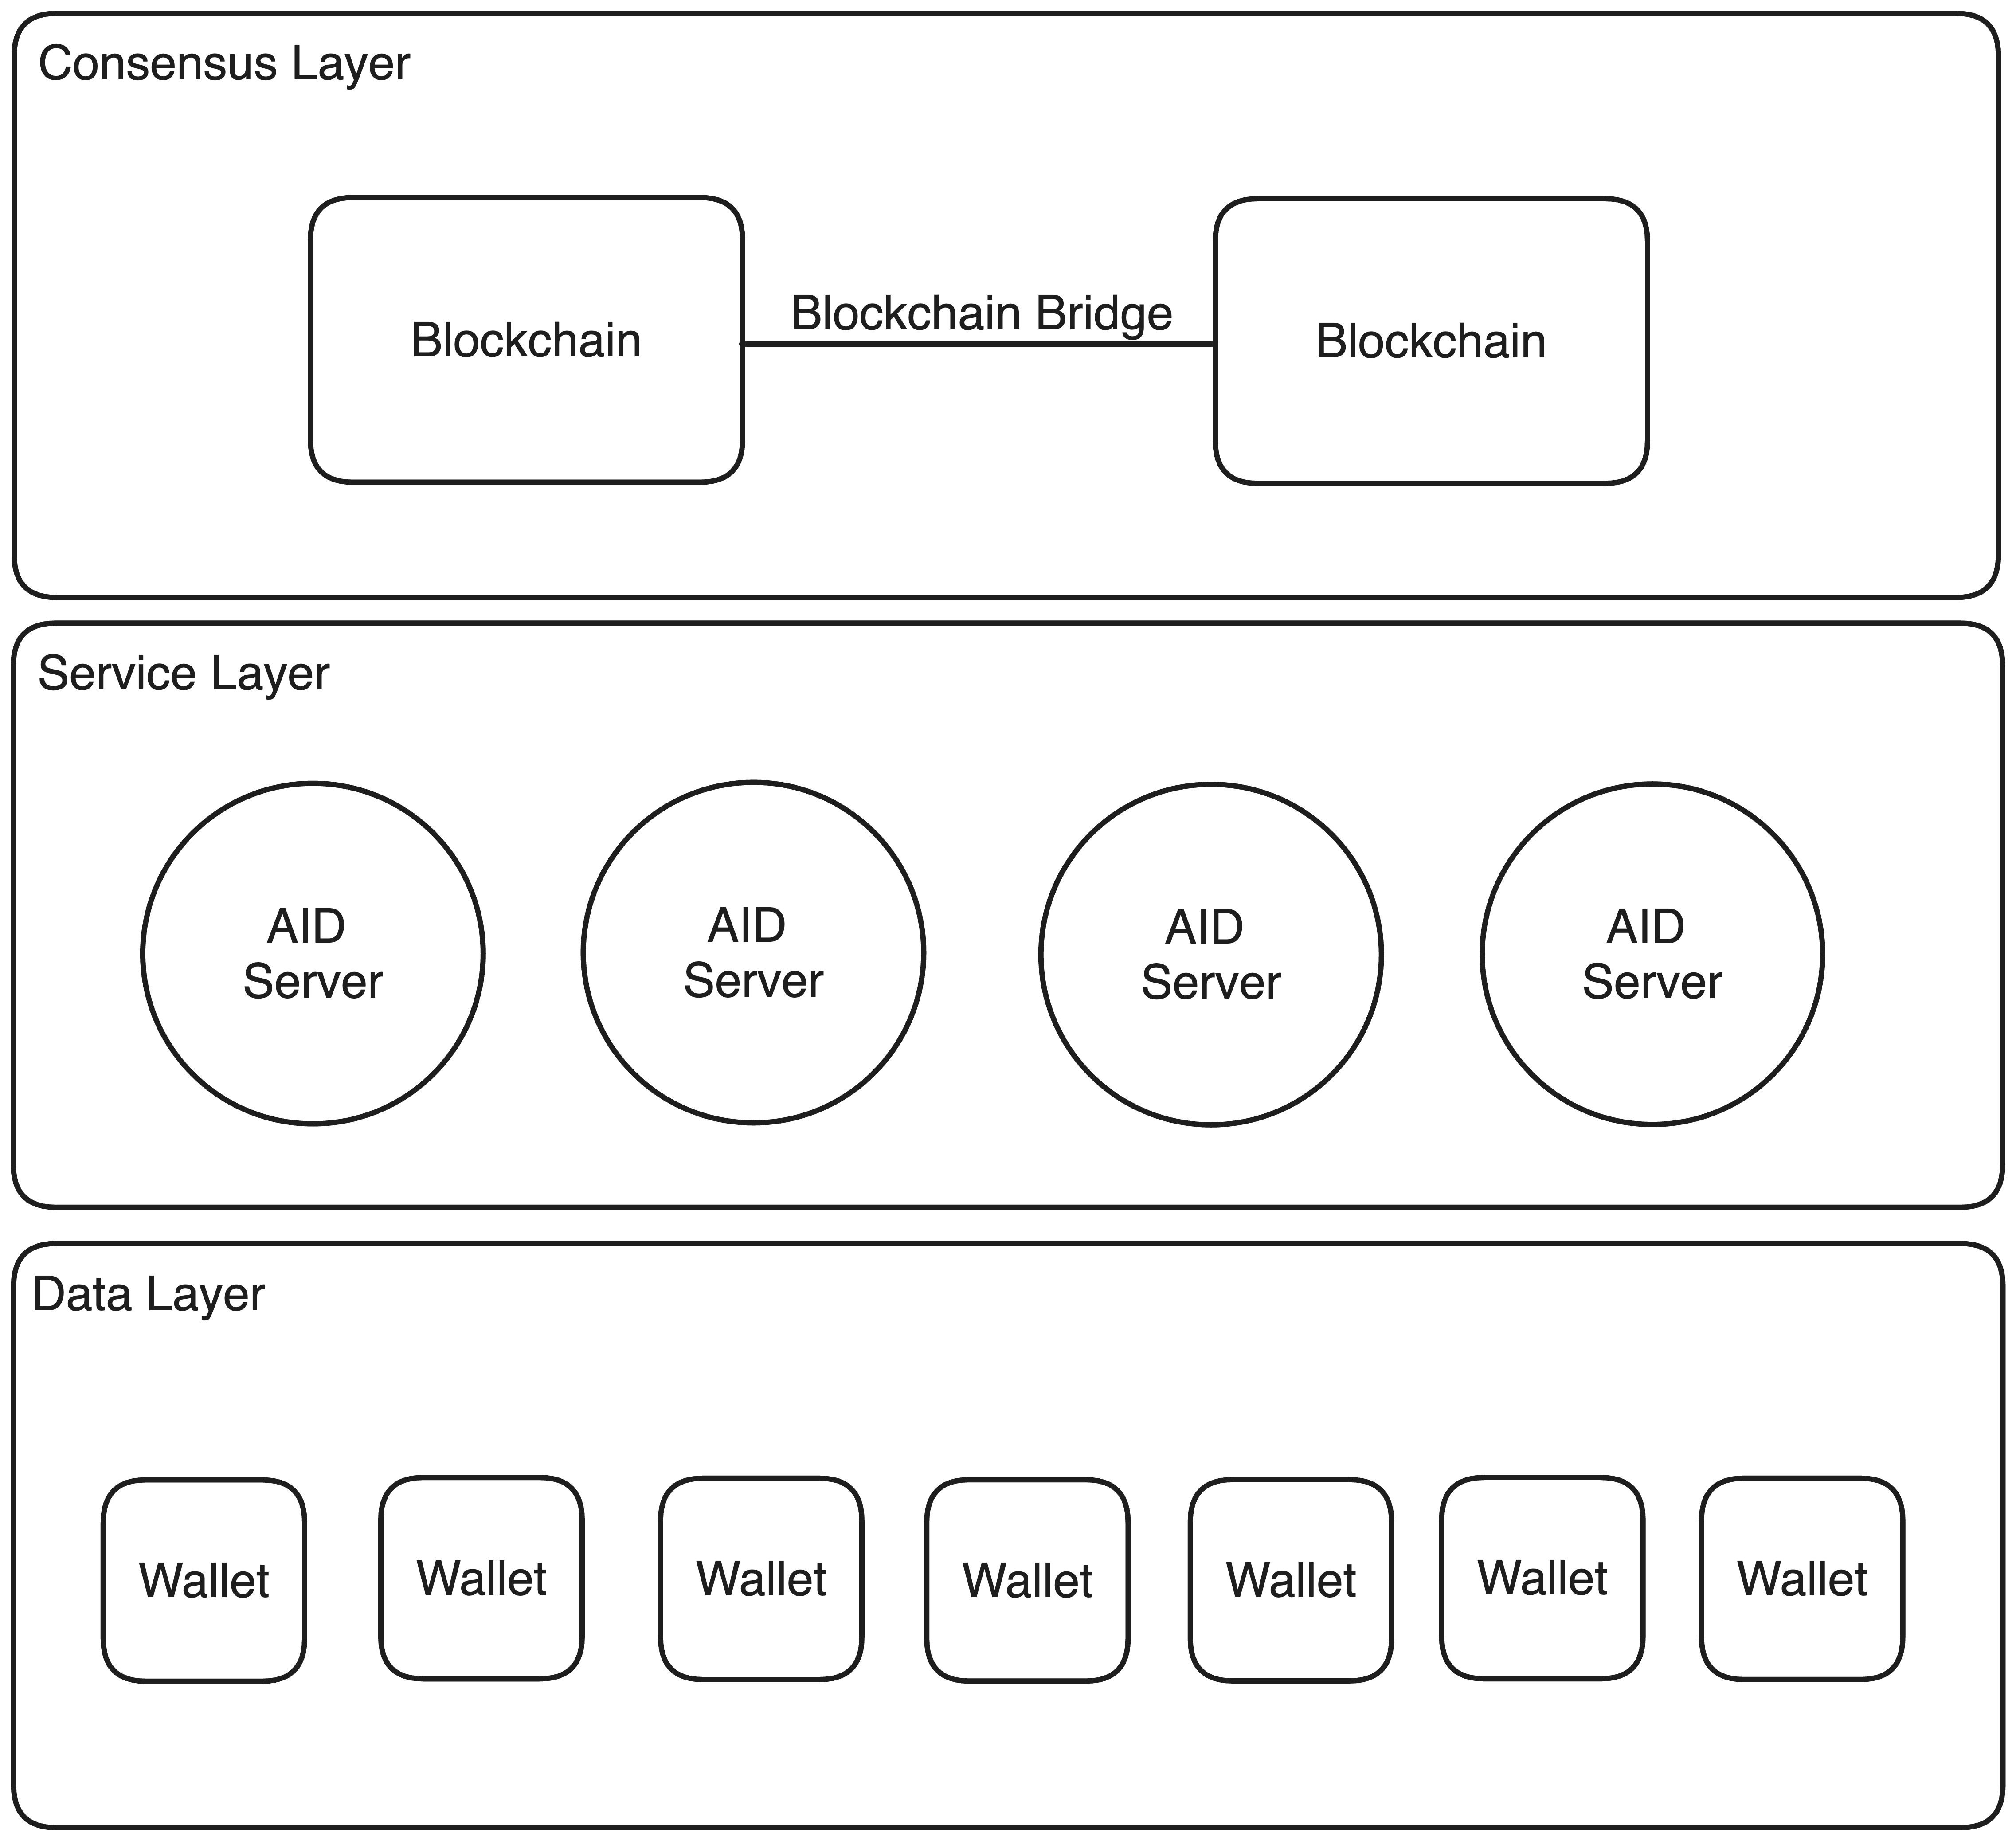
\includegraphics[width=0.8\textwidth]{figures/aidLayers.png}
  \caption{自主身份系統分層架構}
  \label{fig:aid-layers}
\end{figure}

更深入地看,共識層的核心組成是具備共識機制的區塊鏈系統。這一層級可通過跨鏈橋等先進機制實現水平擴展,顯著提升系統的可擴展性。區塊鏈中的智能合約扮演著關鍵角色,它為服務層和數據層提供了對共識數據進行讀寫操作的介面。值得注意的是,共識層的實現並不局限於區塊鏈技術。在存在可信第三方機構的情況下,其他形式的共識機制同樣可以被採用,這為系統設計提供了更大的靈活性。

服務層由多樣化且相互獨立的網路服務構成,這些服務可能以移動應用、網站或API服務等形式呈現。儘管各服務的具體需求可能大相徑庭,但它們都需要強大的身份管理功能。為了滿足這一普遍需求,我們提出了一個統一的解決方案:AID Server。我們設計了一個用於多種程式語言的後端SDK規格,它在保留客製化空間的條件下為服務提供者提供了一個標準化的身份管理介面。通過AID Server,服務開發者能夠輕鬆地實現與共識層和數據層的無縫對接,大大簡化了開發流程並維持了系統的一致性。

數據層主要由大量獨立的終端應用組成,這些應用可能是智能手機APP、個人電腦軟體或物聯網(IoT)設備等。與服務層類似,數據層中的應用雖然功能各異,但都需要可靠的身份管理能力。針對這一需求,我們設計了名為Wallet的前端SDK規格。Wallet能在多種程式語言下為應用開發者提供統一的身份管理介面。這使得開發者能夠輕鬆地實現數據層應用與共識層和服務層的有效對接,從而構建出一個完整且高效的生態系統。

這種多層架構設計不僅確保了系統各部分的模組化和解耦,還提高了整體系統的可擴展性、靈活性和安全性。通過標準化的介面和SDK規格,我們大大降低了開發難度,同時提高了不同層級間的互操作性。接著,我們將進一步介紹各層的的具體規格與設計細節。
\subsection{共識層}
共識層是自主身份系統的基礎建設,主要由無數個智能合約組成。並且,所有智能合約都應該包含以下四個功能,分別介紹:
\begin{itemize}
  \item \textbf{數據寫入:} 將特定格式的數據雜湊寫入區塊鏈,並提供即時的評價與狀態寫入功能。
  \item \textbf{數據讀取:} 讀取區塊鏈上特定數據的雜湊,並獲取相關評價與狀態資訊。
  \item \textbf{狀態更新:} 由證書擁有者執行,用於即時變更證書狀態,如撤銷或停用。
  \item \textbf{評價機制:} 允許使用者根據智能合約規則,以特定格式留下評價內容。
\end{itemize}
為了更好地理解共識層的運作,讓我們以學歷驗證為例。在這個場景中,使用者向學校申請學歷證明,學校將證明的數位簽名寫入區塊鏈。任何需要驗證該學歷的服務都可以通過讀取區塊鏈上的簽名來確認其真實性。若使用者的學歷狀態發生變化,學校可以即時更新區塊鏈上的簽名狀態,確保驗證方獲得最新資訊。此外,如果某企業對學歷證明的可信度存疑,可以在區塊鏈上留下評價,供其他驗證方參考。

為了保障使用者自主權,區塊鏈上寫入的簽名應遵循特定協議的智能合約,讓使用者能自由決定操作簽名的規則。例如,使用者可以選擇具有刪除評價功能的智能合約來承載學歷證明的簽名,從而可以刪除特定的惡意評價。這種機制不僅保障了學歷資訊的即時性與真實性,還確保了使用者對自己數據的控制權。

然而,這樣的設計也面臨著諸多挑戰。首要問題是如何有效評價鏈上簽名,並將其轉化為影響使用者信譽的機制。其次,作為系統信任核心的區塊鏈,其長期穩定運營的可行性也是一個極需解決的問題。最後,在跨服務的使用者數據變化過程中,如何建立有效的共識機制同樣是一個關鍵議題。這些新架構下衍生的問題都需要深入探討和研究,以確保系統的可靠性和可持續性。

為了解決評價問題,我們必須理解為何在自主身份系統中,使用者需要在區塊鏈上的簽名留下評價。這涉及去中心化自治組織(DAO)的概念,我們可以將整個自主身份系統視為一個大型自治組織。在這個組織中,每個自主身份(AID)都是成員,每個成員都有信任和被信任的需求。傳統的中心化身份系統中,這種需求是由中心化的身份服務提供者來滿足的。而在自主身份系統中,這種需求則是通過區塊鏈上的評價來滿足。因此,我們可以將評價視為一種投票,其結果直接反映使用者的信譽。

值得注意的是,不僅使用者之間需要建立信任,使用者與服務之間也同樣需要。這種雙向信任的建立主要通過彼此評價來實現。因此,評價成為自主身份系統中的一個核心機制。評價機制的設計需要考慮諸多因素,如評價的權重、範圍和內容如何設定等。這些都涉及實際使用者的需求,我們希望保留使用者的自主權,讓他們可以自由選擇不同協議的智能合約作為區塊鏈上的評價機制。至於智能合約協議的協調與自治,我們期望能夠通過 DAO 中統治代幣的概念來實現。

作為系統信任核心的區塊鏈如何運營,這涉及到區塊鏈的經濟模型。我們提議在區塊鏈中發行一種逐漸增加的自主身份統治代幣。這種代幣可被抵押用於創建使用者的自主身份,藉此防止惡意使用者大規模創建惡意帳戶。每個自主身份(相當於其背後的代幣)可參與定期投票,討論評價機制的調整、新的智能合約協議等議題。為確保區塊鏈的長期運作,我們建議對失去信任的使用者實施懲罰,同時獎勵基礎設施的運作。因此,用於創建自主身份的代幣抵押後不可贖回,而是被鎖定在區塊鏈上。這樣可以確保使用者不會輕率創建自主身份,並激勵使用者維護自身自主身份的信譽。此外,我們建議對使用者在鏈上的每項操作採取使用者付費模式,使區塊鏈的維護者能獲得報酬,從而保證區塊鏈的持續運作。

最後,我們需要設計一個機制來實現跨服務的使用者數據變化共識。這是一個常見的網路服務需求,如微服務間的調用即為典型案例。在我們的設計中,資料的控制權從服務提供者轉移到使用者身上,這將大幅改變當前網路後端應用的設計。基於共識層的功能,我們提議讓使用者成為多個服務之間的橋樑。具體而言,使用者在區塊鏈外傳遞特定格式的資訊,而服務提供者則在區塊鏈上驗證這些資訊,從而達成共識。

舉例來說,實作一個使用第三方支付服務的購票系統時,我們的方法與現行的網路後端設計有所不同。現有設計中,購票系統全權負責與支付體系的串接,使用者僅需與購票系統溝通。而在我們提出的架構下,流程如下:
\begin{enumerate}
  \item 購票系統要求使用者到銀行服務完成支付並取得收據。
  \item 銀行服務將收據的簽名寫入區塊鏈。
  \item 使用者向購票系統提交收據和購買請求。
  \item 購票系統在區塊鏈上驗證收據的真實性。
  \item 驗證通過後,完成購票流程。
\end{enumerate}
這種方式不僅確保了數據的可信度,還賦予了使用者更多對自身數據的控制權,體現了自主身份系統的核心理念。
\subsection{服務層}
服務層是自主身份系統的應用層,負責提供各種服務。自主身份系統不包含具體服務的實作,只是提供名為AID Server的後端SDK規格,讓服務開發者能夠輕鬆地把自己的應用接入自主身份系統。我們設計了AID Server的幾個關鍵功能:
\begin{itemize}
  \item \textbf{身份管理:} 提供服務註冊、登入、登出等基本身份管理功能。
  \item \textbf{證書管理:} 提供共識證書的創建、更新、讀取、評價等功能。
  \item \textbf{數據管理:} 提供使用者數據的導入、導出等功能。
\end{itemize}
以下將分別介紹這幾個功能的設計細節。
\subsubsection{身份管理}
對服務提供者而言,新的自主身份註冊必須提供基於「自主證書」機制創建。此時,服務提供者可選擇是否接受該新自主身份。多數公開服務可能接受任何自主身份,但私人服務或有更高要求,如僅接受特定機構簽章的自主證書,或基於評價機制被充分信任的自主身份。一旦服務提供者接受新的自主身份,該身份即可開始使用服務。

為了在確保安全的同時提供便利,自主身份系統提供了兩種登入方式:簡易登入和多因素驗證登入。簡易登入是指使用者僅需提供少量資訊即可登入,如使用者別名和密碼。多因素驗證登入則要求使用者提供更多資訊,如電子郵件驗證碼、手機簡訊驗證碼或私鑰等。服務提供者可根據自身需求選擇是否啟用簡易登入功能。

另外,儘管自主身份(AID)的生成是透過 UUID 機制\cite{uuid}產生唯一識別號,但AID系統允許使用者在服務中設定自己偏好的別名,而非如傳統身份服務限制使用唯一的電子郵件地址作為使用者名稱。在日常操作中,系統優先讓使用者使用別名作為帳號完成簡易登入,只有當別名因難以被識別時,才會要求使用者使用與 UUID 關聯的多因素驗證登入機制進行識別。

然而,此設計亦面臨諸多挑戰。首要問題是當使用者採用簡單方案登入時,可能因提供資訊不足而被攻擊者冒充或無法成功辨識身份。為此,我們提出「基於使用者時空的分析方法」作為系統性解決方案,通過追蹤使用者每次操作時夾帶或產生的資訊來辨識使用者身份,並配合「基於危險程度的驗證機制」找出應要求多因素驗證的時機。此設計在保留使用者便利性的同時,亦確保了安全性。

另一挑戰是如何在自主條件下,協助使用者處理忘記密碼的情況。自主身份應包含「極致多因素認證」概念,允許使用者在創建自主證書時設置多種驗證方案,包括難以遺失或忘記的方法,如生物特徵識別(指紋或臉部辨識)。如此,即使使用者忘記密碼,亦可通過這些驗證方式重新取回身份。進一步擴展此方案,我們可將「極致多因素認證」概念應用於「基於危險程度的驗證機制」,根據危險程度要求使用者使用多種方法完成多因素驗證,進一步提高安全性。

會在資安分析的章節中詳細說明「基於使用者時空的分析方法」與「基於危險程度的驗證機制」等特殊解決方案。
\subsubsection{證書管理}
證書管理在自主身份系統中扮演著雙重角色:一方面對使用者自主身份的證書進行操作,另一方面為實現「數據證書」機制而對證書進行操作。

系統可通過讀取區塊鏈上使用者身份證書的狀態與簽名來完成身份驗證。此外,其他實體(如服務提供者或其他使用者)可基於自身經歷,在使用者證書對應的鏈上合約中留下評價。這樣的設計不僅有助於使用者在不同服務間建立信任,還能讓服務提供者更全面地了解使用者的信譽狀況。

在「數據證書」方面,當使用者申請共享特定數據時,服務提供者可按照預定的智能合約協議創建證書,並將證書簽名發布到區塊鏈上。如果數據發生變動,服務提供者可即時更新證書狀態,確保使用者數據的即時性和真實性。當另一個服務收到使用者在區塊鏈外提交的完整證書後,除了可以通過區塊鏈上的簽名驗證證書的真實性外,還可以在區塊鏈上留下評價,為其餘服務提供者提供參考。
\subsubsection{數據管理}
數據管理在服務層相對簡單,因為自主身份系統的核心在於賦予使用者控制自身數據的權利。理論上,服務提供者的最低要求是確保使用者能夠:
\begin{enumerate}
  \item 將當次操作所需的數據導入服務中
  \item 在操作結束後將數據導回使用者端
\end{enumerate}
然而,這種簡單設計可能大幅降低使用者體驗。例如:
\begin{itemize}
  \item 若使用者每次操作都需要導入和導出數據,許多優化使用者體驗的功能將變得不可行,因系統無法追蹤使用者歷史數據。
  \item 頻繁的大量數據導入導出會顯著增加操作延遲和網路成本。
\end{itemize}
因此,「混合數據管理」模式成為必然選擇,即部分數據由使用者保管,部分由服務提供者保管。這種設計在保護使用者隱私的同時,也確保了操作的便利性。
然而,「混合數據管理」模式仍面臨諸多需要服務提供者與使用者達成共識的問題,包括:
\begin{itemize}
  \item 哪些數據由使用者管理?
  \item 哪些數據由服務提供者管理?
  \item 服務提供者管理的數據保留時間?
  \item 數據的使用權限?
\end{itemize}
這些問題涉及對隱私和資安的權衡。為確保使用者自主權,我們建議:
\begin{enumerate}
  \item 採用逐步詢問的方式協助使用者設定所有簡化的資安措施或降低的隱私保護措施。
  \item 設置應從高到低、從嚴格到寬鬆平滑過渡,使使用者能根據自身需求調整安全性和隱私保護程度。
\end{enumerate}
這種方法能在保護使用者權益的同時,為服務提供者提供必要的數據支持,實現雙方利益的平衡。透過這種「混合數據管理」模式,我們可以在自主身份系統中實現數據的高效管理,同時保障使用者的數據主權。
\subsection{數據層}
數據層是自主身份系統的存儲層,負責存儲使用者個人數據。我們設計了名為Wallet的前端SDK規格,讓數據層應用開發者能夠輕鬆地把自己的應用接入自主身份系統。Wallet的幾個關鍵功能如下:
\begin{itemize}
  \item \textbf{身份管理:} 提供自主身份的註冊功能。
  \item \textbf{數據管理:} 提供使用者數據的上傳、下載等功能。
  \item \textbf{證書管理:} 對共識簽名的更新、讀取、評價等功能。
  \item \textbf{數據存儲:} 儲存使用者的數據。(數據備份, 數據遷移, 雲端暫存, ......)
\end{itemize}
以下將分別介紹這幾個功能的設計細節。
\subsubsection{身份管理}
Wallet 的身份管理主要提供一個核心功能:註冊自主身份。這裡的註冊並非指使用者加入某個服務,而是包含兩個主要功能:
\begin{enumerate}
  \item 使用者直接在本地裝置透過隨機產生的 UUID 創建自己的自主身份
  \item 透過「自主證書機制」創建新的證書
\end{enumerate}
在我們的設計中,使用者可依據需求使用個人裝置創建不同的自主身份,並為不同需求生成不同的身份證書,再利用這些證書與不同的服務進行互動。當使用者需要向服務證明自己是證書的真實持有者時,僅需透過 Wallet 完成證書上標示的多因素驗證方案。
\subsection{數據管理}
Wallet 的數據管理功能主要在服務需要時,將特定數據自主上傳至服務中,並在服務結束後自主下載回本地裝置。這裡的「自主」指使用者可自由選擇是否上傳或下載數據,並可自由選擇上傳或下載的數據內容。這樣的設計不僅更徹底地保護了使用者的安全與隱私,更徹底解決了數據孤島的問題。

在 Wallet 中,使用者可統一儲存所有個人數據。當服務有需要時,透過 Wallet 提供的 API 進行資料的上傳與下載。這樣的介面配合「數據證書」與「自主證書」機制,還能解決許多使用者隱私權中的難題,如:
\begin{itemize}
  \item \textbf{被遺忘權}:當使用者希望遺忘數據時,可直接清除個人保留的數據。區塊鏈中僅保留簽名,而不保留數據本身。理論上,服務內部不會存儲使用者數據;即使確實存儲了,由於唯一能證明數據擁有人的是使用者本身,因此相當於使用者與數據無關。這個概念類似於 Cameron\cite{cameron2005laws}所描述的單向身份:使用者可以通過個人證明指向自己的數據,但僅有數據無法指向使用者。
  \item \textbf{積極數據授權}:採用類似「自主證書」的方法,使使用者與服務提供者對數據授權產生明確共識。當使用者授權服務提供者使用數據時,會對數據與使用範圍生成證書,並上傳對應簽名至區塊鏈,然後將證書與數據傳送給服務提供者。之後,使用者可利用公開證書證明數據被濫用,反之,服務提供者也可利用公開證書證明數據被合法使用。這樣的設計使使用者與服務提供者之間的數據授權變得更加明確且公平。
\end{itemize}
\subsubsection{證書管理}
Wallet 的證書管理功能主要對共識層內證書簽名進行更新、讀取、評價等操作。基於「數據證書」與「自主證書」機制,使用者與服務需要在共識層中的區塊鏈上基於智慧合約留下證書簽名,讓人們可在區塊鏈上驗證證書的真實性。此外,所有使用者(包含服務提供者)都可在區塊鏈上對智能合約進行操作,以留下評價,藉此形成共識達成信任。

在 Wallet 中實作的證書管理功能,使用者可輕易從 Wallet 中直接讀取共識層內的信任關係,並直接在共識層中更新自己身份證書簽名的狀態,以及對他人或服務的證書簽名進行評價。這樣的設計不僅提高了使用者的自主權,更讓使用者能更直接地參與共識層的運作。
\subsubsection{數據存儲}
Wallet 的數據存儲功能主要用於儲存使用者的各類數據,包括證書、公私鑰、個人資料以及與各服務的交互紀錄等。這種設計使 Wallet 成為使用者的個人化數據中心,實現統一管理。然而,將個人移動設備轉化為數據中心需解決備份、遷移和雲端儲存等問題。雖然我們鼓勵使用者自主選擇解決方案,但仍提供以下建議實作:

每個採用自主身份系統的應用都應包含 Wallet 模塊,並利用設備的嵌入式資料庫存放數據。使用者可設置各 Wallet 的同步策略,包括自動同步(按需獲取數據)、完全同步(複製全部使用者數據)和手動同步(使用者指定數據複製)。這種設計便於實現備份、遷移和雲端儲存等功能,提升使用者數據管理的便利性。具體實現如下:
\begin{itemize}
  \item \textbf{遷移:} 新 Wallet 可通過手動輸入舊 Wallet 的公開地址或直接連接同一設備上的已啟動 Wallet 來建立連結。遷移後,新 Wallet 可設置對舊 Wallet 的同步策略。
  \item \textbf{雲端儲存:} 考慮到在單一移動設備上存儲全部個人數據的安全風險,以及一般使用者難以維護家庭 P2P 集群的現實,專業雲端服務供應商可提供執行完整 Wallet 的服務。使用者支付費用後,可使其他 Wallet 連接到此雲端 Wallet。
  \item \textbf{備份:} 當使用者在多個設備上維護多個 Wallet,並重複存儲每項數據時,自然形成了數據備份機制。
\end{itemize}
這種多元化的數據管理策略不僅提高了數據安全性,也增強了系統的靈活性和使用者體驗。
\section{資料結構}
\subsection{AID Server}
\subsection{Wallet}
\subsection{Consensus Core}
\section{資安分析}
\subsection{基於使用者時空的分析方法}
每個身份本質上可視為一個隨時間變化的動態向量空間,其維度可謂無窮。每次對使用者的身份驗證都可視為取得特定時間僅含部分維度的向量。這方法的核心是讓使用者自主決定提供哪些維度,並在每次與系統互動時攜帶這些資訊。基於此概念,系統可藉由比對當次傳入的向量和近期暫存在快取中的所有向量來推測使用者的真實身份。

舉例來說:使用者在某次登入時提供了自己的別名、性別、所在地區等資訊,而在下次登入時僅提供了性別、所在地區等資訊,系統可以通過比對這兩次向量來推測使用者的別名。這種方法使使用者在不提供完整資訊的情況下,仍能通過部分資訊完成身份驗證。

然而,這種方法也帶來了一些問題。例如,使用者提供的維度多寡會影響系統的準確性,甚至使用者提供的維度是否包含可變資訊會影響系統的安全性。因此,我們提出維度的選擇甚至各個維度的權重應由使用者自主決定,而系統僅提供推薦機制。這樣可讓使用者在不同情境下使用不同方法,以滿足其需求。

總的來說,當僅有一個使用者被比較出來時視為可識別,有零個或多個使用者被比較出來時視為不可識別。這種機制受比較方法影響,因此我們提出了「基於危險程度的驗證機制」,希望能在不同情境下選擇適合的比較方法。
\subsection{基於危險程度的驗證機制}
此機制主要使用在比較身份與歷史紀錄時選擇適合的比較方法。不同的比較方法可能導致不同的結果,因其本質上代表了不同的嚴謹程度。在嚴謹程度較高的情況下,使用者可能需要更多維度符合,或需要在更接近的時間點內提供的紀錄才算數。這可能導致使用者難以找到識別對象,進而要求補充更多資訊再次驗證。相反,在嚴謹程度較低的情況下,使用者可能僅用少量維度的資訊配合較遠時間點的紀錄來完成驗證,這可能導致使用者被誤認為其他使用者,威脅系統安全。

考慮使用者行為的危險程度,我們設計出以下規則:
\begin{enumerate}
  \item 當使用者的行為被視為危險時,系統應提高驗證的嚴謹程度。
  \item 當使用者的行為被視為安全時,系統應降低驗證的嚴謹程度。
\end{enumerate}

接著,我們將嚴謹程度拆分為時間和空間兩個軸,使用笛卡爾座標系統表示,以細分出更複雜的情境:
\begin{enumerate}
  \item 當使用者行為超危險時,比較標準應為時間非常近或多個維度符合。
  \item 當使用者行為危險時,比較標準應為時間相對近或維度相對符合。
  \item 當使用者行為安全時,比較標準應為時間相對遠或維度相對不符合。
  \item 當使用者行為超安全時,比較標準應為時間非常遠或僅幾個維度符合。
\end{enumerate}

最後,使用者行為的危險程度在我們的系統中是由使用者自主決定的,系統僅提供推薦機制。我們希望藉此滿足所有使用者在各種情境下的需求。例如,對於個人銀行帳戶,可能所有行為都視為最高危險,因此需要最高的驗證嚴謹程度。而對於個人社群帳戶,讀取文章的行為可能視為不危險,發布文章則視為危險,因此需要不同的驗證嚴謹程度。我們建議使用者將危險的概念定義為對使用者數據變動的敏感程度:越敏感的數據越危險,越危險的數據越需要嚴謹的驗證機制。
\section{本章總結}
系統如何解決所有缺點,並且保留所有優點。
